\documentclass{standalone}

\renewcommand{\familydefault}{\sfdefault}
\usepackage{amsmath}
\usepackage{tikz}
\usetikzlibrary{arrows.meta, positioning, calc, }

\newcommand{\quadrup}[5]{%
  % #1 = x, #2 = y, #3 = largura, #4 = altura, #5 = cor
  \fill[#5]
    (#1-0.5*#3,#2+0.5*#4) --
    (#1,#2) --
    (#1+0.5*#3,#2+0.5*#4) --
    cycle;
  \fill[#5]
    (#1-0.5*#3,#2-0.5*#4) --
    (#1,#2) --
    (#1+0.5*#3,#2-0.5*#4) --
    cycle;
}

\newcommand{\bpmrule}[6]{%
  % #1 = x_inicial, #2 = altura total H, #3 = número de marcas, #4 = cor
  \draw[#4, thick] (#1,-0.5*#2) -- (#1,0.5*#2);
  \foreach \x in {1,...,#3} {
    \pgfmathparse{\x == #5 ? 1 : 0}
    \ifnum\pgfmathresult>0\relax
      \draw[#4, thick] (#1, 0.5*#2 - #2*\x/#3 + 0.5*#2/#3)
                    -- ++(0.2,0) node[right, xshift={-0.25em}] {\footnotesize 0};
    \else
      \pgfmathparse{mod(\x - #6,5) == 0 ? 1 : 0}
      \ifnum\pgfmathresult>0\relax
        \draw[#4, thick] (#1, 0.5*#2 - #2*\x/#3 + 0.5*#2/#3)
                    -- ++(0.2,0);
      \else
        \draw[#4, line width=0.65pt] (#1, 0.5*#2 - #2*\x/#3 + 0.5*#2/#3)
                      -- ++(0.1,0);
      \fi
    \fi
  }
}

\begin{document}

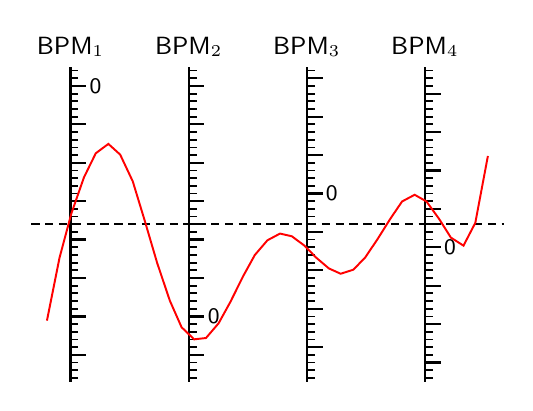
\begin{tikzpicture}[>=latex]
    \coordinate (O) at (0, 0);
    
    \draw[thick, densely dashed] (-4, 0) -- (2, 0);

    % \draw[line width=0.7pt, red, -stealth] ($1.7*(B)$) -- ($-1*(B)$) node[right, yshift={-0.25em}] {\small{beam}};

    \bpmrule{-3.5}{4}{41}{black}{3}{-2}
    \node[above, black] at (-3.5, 2) {\small{BPM$_1$}};

    \bpmrule{-2}{4}{41}{black}{33}{3}
    \node[above, black] at (-2, 2) {\small{BPM$_2$}};

    \bpmrule{-0.5}{4}{41}{black}{17}{2}
    \node[above, black] at (-0.5, 2) {\small{BPM$_3$}};

    \bpmrule{1}{4}{41}{black}{24}{-1}
    \node[above, black] at (1, 2) {\small{BPM$_4$}};

    \draw[line width=0.7pt, red, yscale={1.7}] (-3.80, -0.72) -- (-3.64, -0.25) -- (-3.49, 0.08) -- (-3.33, 0.35) -- (-3.18, 0.53) -- (-3.02, 0.60) -- (-2.87, 0.52) -- (-2.71, 0.32) -- (-2.56, 0.03) -- (-2.40, -0.29) -- (-2.24, -0.57) -- (-2.09, -0.77) -- (-1.93, -0.86) -- (-1.78, -0.85) -- (-1.62, -0.74) -- (-1.47, -0.58) -- (-1.31, -0.39) -- (-1.16, -0.23) -- (-1.00, -0.12) -- (-0.84, -0.07) -- (-0.69, -0.09) -- (-0.53, -0.16) -- (-0.38, -0.25) -- (-0.22, -0.33) -- (-0.07, -0.37) -- (0.09, -0.34) -- (0.24, -0.25) -- (0.40, -0.11) -- (0.56, 0.04) -- (0.71, 0.17) -- (0.87, 0.22) -- (1.02, 0.17) -- (1.18, 0.04) -- (1.33, -0.10) -- (1.49, -0.16) -- (1.64, 0.01) -- (1.80, 0.51);

\end{tikzpicture}


\end{document}

% \documentclass{standalone}

% \usepackage{amsmath}
% \usepackage{tikz}
% \usetikzlibrary{arrows.meta, positioning, calc, }

% \begin{document}

% \begin{tikzpicture}[>=latex]
%     \coordinate (O) at (0, 0);
%     \coordinate (A) at (-2, 0.3);
%     \coordinate (B) at (-1, -0.7);
%     \coordinate (C) at (0, 0.1);
%     \coordinate (D) at (1, 0.5);

%     \pgfmathsetmacro{\blarg}{0.2}
%     \pgfmathsetmacro{\balt}{0.4}
    
%     \path[fill=black!60, draw=none] ($(A)+(\blarg/2,\balt/2)$) rectangle ($(A)-(\blarg/2,\balt/2)$);
%     \node[above] at ($(A)+(0,\balt/2)$) {\tiny BPM$_1$};
    
%     \path[fill=black!60, draw=none] ($(B)+(\blarg/2,\balt/2)$) rectangle ($(B)-(\blarg/2,\balt/2)$);
%     \node[above] at ($(B)+(0,\balt/2)$) {\tiny BPM$_2$};

%     \path[fill=black!60, draw=none] ($(C)+(\blarg/2,\balt/2)$) rectangle ($(C)-(\blarg/2,\balt/2)$);
%     \node[above] at ($(C)+(0,\balt/2)$) {\tiny BPM$_3$};

%     \path[fill=black!60, draw=none] ($(D)+(\blarg/2,\balt/2)$) rectangle ($(D)-(\blarg/2,\balt/2)$);
%     \node[above] at ($(D)+(0,\balt/2)$) {\tiny BPM$_4$};
    
%     \draw[thick, ->] (-3, 0) -- (2, 0) node[right] {$s$};
%     \draw[thick, ->] (-2.8, -1) -- (-2.8, 1.5) node[above] {$x$};

% \end{tikzpicture}


% \end{document}